TL;DR: Wir konnten fast all unsere Anforderungen erfüllen.

\section{KZO}
% \includegraphics[height=18cm]{resources/diagrams/use-case}
\begin{enumerate}
    \item \textbf{Zeit} \\
        Geplant war ungefähr eine Lektion pro Woche. Wir haben die geschätzten 50 Stunden um einen Faktor von sechs überschritten. Unser gemessener Zeitaufwand, während aktivem Programmieren,
        beträgt über 330 Stunden. Da sind die Stunden, in denen wir uns in der Freizeit, und mit Herrn Hunziker getroffen haben, gar nicht notiert.
    \item \textbf{Begleitperson} \\
        Wir hatten zum Glück kein Problem eine Begleitperson zu finden. Martin Hunziker war gerne bereit unsere Arbeit im Blick zu behalten.
    \item \textbf{Plagiat} \\
        Zwar sind einige Grafiken aus dem Internet, jedoch sind alle Nutzungsfrei. Auch sonst haben wir keinen Code geklaut und verwendet. 
\end{enumerate}

\subsection*{Notwendig}
\begin{itemize}
    \item \textbf{System} \\
        Unser Spiel funktioniert sowohl auf macOS als auch auf Windows. Dies ausserdem mit einer FPS von 300, bis teilweise 500, bei den meisten modernen Geräten
    \item \textbf{Benutzeroberfläche} \\
    \begin {itemize}
        \item \textbf{Startpage} \\
            \\
            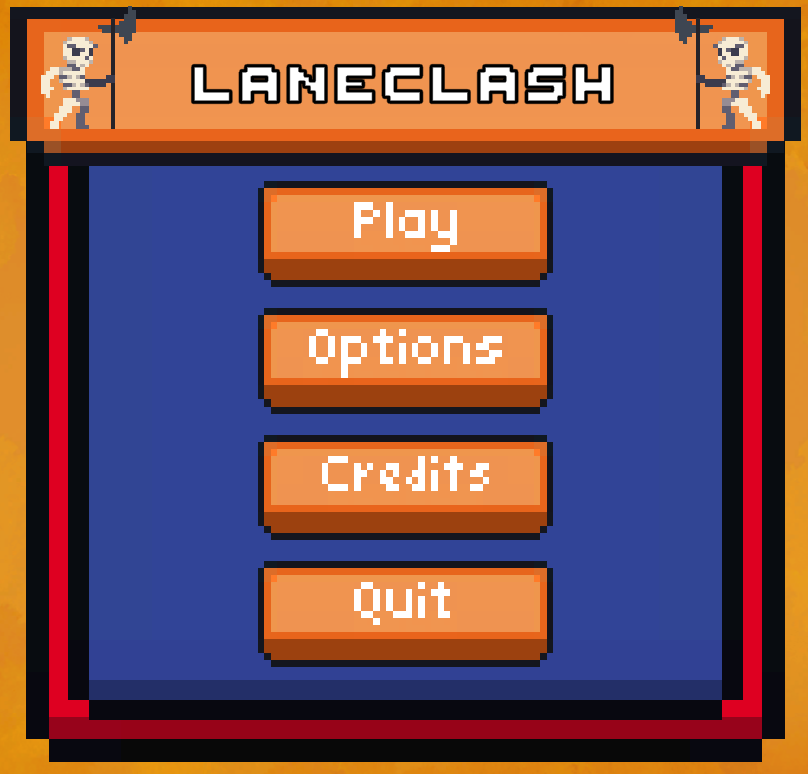
\includegraphics[height=7cm]{resources/laneclash.png}\\
            Unsere Startseite hat einen ''Spielen''-Knopf, einen ''Einstellungen''-Knopf, einen ''Credits''-Knopf und einen ''Verlassen''-Knopf. Unsere vereinzelten Tester bewerteten die Startseite
        als intuitiv verständlich. Bedienbar mit der Maus, hatten die Tester keine Probleme sich zurechtzufinden.
        \item \textbf{Credits}\\
            \\
            \includegraphics*[width = 7cm]{resources/credits.png}\\
            Es gibt die Möglichkeit die Credits vorzeitig zu Verlassen. Dies geschieht durch das Drücken des Knopfes mit dem Haus als Icon. Die Tester fanden dies auch sehr intuitiv.
        \item \textbf{Settings}\\
            \\
            \includegraphics*[height=7cm]{resources/setting.png}\\
            Man kann hier die Auflösung ändern und auswählen, ob das Spiel im Vollbild dargestellt werden soll. Auch gibt es hier die Möglichkeit die Musik lauter, leiser zu stellen
            oder zu muten. Wenn man Einstellungen geändert hat, muss man dies bestätigen. \\
            \includegraphics*[height=3cm]{resources/resolution.png}\\
            Wenn man die Auflösung ändert und dies bestätigt, werden die Änderungen angewendet und man hat zehn Sekunden Zeit erneut zu bestätigen. Sonst werden die Änderungen zurückgesetzt.
            Dies wurde implementiert, um eventuellen Problemen vorzubeugen. 
        \item \textbf{Server Management}\\
            \\
            \includegraphics*[height = 3cm]{resources/server.png}\\
            Nach Interaktion mit dem ''Start''-Knopf gibt es die Möglichkeit einen Server zu Hosten oder einer bereits existierenden Lobby als Client beizutreten. Ausserdem kann man
            automatisch nach bereits existierenden Servern suchen.\\
            \\
            \includegraphics*[width=6cm]{resources/discovered.png}\\
            Den gewollten Server kann man mit einem einfachen Linksklick auswählen.
        \item \textbf{Lobby Management}\\
            \\
            \includegraphics*[width = 5cm]{resources/lobby.png} \includegraphics*[width=5cm]{resources/lobbyc.png}\\
            Player (1) ist dabei immer der Host, und Player (2) immer der Client. Das eigentliche Spiel beginnt erst, sobald beide Spieler bereit, also ''ready'', sind. 
            Dieser Status ''ready'' wird dabei immer aktualisiert dargestellt. Der Host hat ausserdem die Möglichkeit den Spieler (2) aus der Lobby zu entfernen. Wir wollten zuerst
            eine Möglichkeit für einen ''Schlüssel'' hinzufügen, allerdings stellte sich dies als überflüssig heraus, da alle Spieler unter einem Dach sitzen.
        \item \textbf{InGame-UI}\\
            \\
            \includegraphics*[height=2cm]{resources/returnlobby.png} \includegraphics*[height=2cm]{resources/stopclient.png}\\
            Der Host hat im Spiel die Möglichkeit, den Server zurück zur Lobby zu schicken, und das Spiel somit neuzustarten. Er kann auch direkt aufhören zu hosten. 
            Auch der Client hat durchgehend die Möglichkeit den Server zu verlassen.\\
            \\
            \includegraphics*[height=2cm]{resources/pause.png}\\
            Im Pausemenu kann man ausserdem auf die Schnelle die Musiklautstärke und die Stärke des Schneefalls ändern.


    \end {itemize}

    \item \textbf{Lokaler Multiplayer} \\
        Das Spiel kann im lokalen Netz gespielt werden. Zum Testen auch auf demselben Gerät. Als Protokoll haben wir TCP gewählt. Dies, da TCP viel zuverlässiger ist.
        Folgende vier Punkte waren entscheidend für die Wahl von TCP über UDP:
        \begin{itemize}
            \item \textbf{Zuverlässigkeit}\\
                Keine Probleme mit verloren gegangenen Paketen. Ging ein Paket verloren, sendet TCP es einfach erneut. Entweder werden alle Daten erfolgreich übermittelt,
                oder man bekommt einen Error.
            \item \textbf{Sequenziert}\\
                TCP stellt sicher, dass jede Nachricht in der gleichen Reihenfolge eintrifft, in der sie gesendet wurde. Wenn man ''a'' dann ''b'' sendet, erhält man auf der
                anderen Seite garantiert auch zuerst ''a'' dann ''b''.
            \item \textbf{Verbindungsorientiert}\\
                TCP hat sich auf das Konzept einer Verbindung konzentriert. Eine Verbindung bleibt so lange offen, bis entweder der Client oder der Server sich dazu entscheiden, sie zu schliessen.
                Anschliessend werden sowohl Client als auch Host benachrichtigt, dass die Verbindung beendet wurde.
            \item \textbf{Überlastungskontrolle} \\
                Wenn ein Server überlastet wird, drosselt TCP selbstständig die Daten, um einen Zusammenbruch durch Überlastung zu verhindern.


        \end{itemize}
    \item \textbf{Einstellungen} \\
        Auflösung, Vollbild, Lautstärke und Stärke des Schneefalls können eingestellt werden.
    \item \textbf{Kamera} \\
        Die Kamera ist beweglich und das ganze Schlachtfeld ist sichtbar. Dabei kann man auch zoomen. Kontrollierbar ist dies mit den Pfeiltasten.
    \item \textbf{Truppen} \\
        IMPORTANT\\
        IMPORTANT\\
        IMPORTANT\\
        IMPORTANT\\
        IMPORTANT\\
        IMPORTANT\\
        IMPORTANT\\
        IMPORTANT\\
        IMPORTANT\\
        IMPORTANT\\
        IMPORTANT\\
        IMPORTANT\\
        IMPORTANT\\
        IMPORTANT\\
        IMPORTANT\\
        IMPORTANT\\
        IMPORTANT\\
    \item \textbf{Gewinnmöglichkeit} \\
        Um zu Gewinnen, muss eine eigene Truppe die Portale des Gegners durchschreiten. Dies verhindern zuerst sogenannte Helden. Sterben jene Helden, erledigt ihr Racheeffekt die
        ganze Linie auf der sich der Held befand.
    \item \textbf{Lanes} \\
        Unser Spiel hat 4 sogenannten Linien (''Lanes''). Diese unterschiedlichen Linien wurden in der Tiefe verschoben.
    \item \textbf{Synchronisation} \\
        Unser Spiel Synchronisiert alle Daten in Echtzeit. Dadurch sehen alle Spieler immer das Gleiche. Wird der Client aus einem unbekannten Grund disconnected kann er versuchen
        sich erneut zu verbinden und der Server wird dann direkt alle Daten synchronisieren. Auch hier hilft und das gewählte Protokoll TCP. Geht ein Paket verloren, wird es automatisch
        erneut gesendet. Dies hilft und dabei, die Synchronisation zu jeder Zeit aufrecht zu erhalten.
    \item \textbf{Crossplay}
        Es ist möglich sich mit einem Windows Rechner und einem macOS Rechner zu verbinden. Allerdings muss dem Spiel dazu die Kommunikation durch die Firewall teilweise erlaubt sein.
        Bei einer eher aggressiveren Firewall wird zudem teilweise der Server-Broadcast geblockt. Dies hätte zur Folge, dass man die Server nicht automatisch finden kann. 
        Verbinden sollte man sich allerdings trotzdem noch können.   
\end{itemize}

\subsection*{Anvisiert}
\begin{itemize}
    \item \textbf{Helden} \\
        Beide Spieler haben im Moment den gleichen Helden. Dies ist ein magischer Turm. Er hat keine Angriffsmöglichkeiten. Allerdings kann er sich passiv heilen und so als eine
        temporäre Grenze zwischen den gegnerischen Truppen und den eigenen Portalen agieren. Die eigenen Truppen werden durch diese Portale hinter den Helden gespawned.
    \item \textbf{Design} \\
        \\
        \includegraphics*[height=5cm]{resources/25d.png} \includegraphics*[height=5cm]{resources/25dtwo.png}\\
        Wir haben uns für ein 2.5d Design entschieden. Dabei ist der Vorteil, dass wir 2d Grafiken benutzen können. Die Sprites werden dabei um 45 Grad gedreht. Auch 
        die Kamera schaut in einem 45 Grad Winkel auf das Geschehen. Dadurch ergibt sich die Illusion einer Perspektive, in der man von der Seite auf das Geschehen schaut. 
    \item \textbf{Deck} \\
        IMPORTANT\\
        IMPORTANT\\
        IMPORTANT\\
        IMPORTANT\\
        IMPORTANT\\
        IMPORTANT\\
        IMPORTANT\\
        IMPORTANT\\
        IMPORTANT\\
    \item \textbf{Truppen}
    \begin{itemize}
        \item \textbf{Nahkampf}
            Eine Truppe mit wenig Reichweite.
        \item \textbf{Fernkampf}
            Eine Truppe die auf Reichweite angreift. Sie scheisst Projektive, zum Beispiel ein Bogenschütze,
            der mit Pfeilen schiesst.
        \item \textbf{Suizid}
            Eine Truppe die bei Berührung mit einem Gegner stirbt und einen Effekt auslöst.
    \end{itemize}
    \item \textbf{Effekte}
    \begin{itemize}
        \item \textbf{Gift:}
            Zeitlich limitierter und wiederholender Schadenseffekt. Eine visuelle Markierung soll vorhanden sein
            und das gleiche Gift, also der gleichen Truppe, soll nur einmal auf jemanden sein. (Hier: Pilz-Truppe)
        \item \textbf{Rache:}
            Truppen mit Rache haben einen Effekt nach ihrem Tod. Zum Beispiel eine Truppe beschwören oder Schaden verursachen. (Hier: Helden mit Feuer)
    \end{itemize}
\end{itemize}

\subsection*{Möglichkeiten}
\begin{itemize}
    \item \textbf{Monetarisierung} \\
    \begin{enumerate}
        \item \textbf{Kostenpflichtiges Spiel}
        \begin{itemize}
            \item Wir haben eventuell vor unser Spiel nach Vollendung der Dev Phase zu veröffentlichen. Allerdings auf keinen Fall für einen hohen Preis.
        \end{itemize}
    \end{enumerate}
    \item \textbf{Design} \\
        Wir werden auch in Zukunft das Design noch verbessern. Hier gehts es aber um den Feinschliff, z.B. mehr Hintergründe, und mehr Dinge selbst zu designen.
    \item \textbf{Truppen}
        Weitere Truppen können jederzeit erstellt werden. Hier ist kein Limit gesetzt. Leben, Schaden, Darstellung, Effekt und vieles mehr kann angepasst werden. 
        Wir haben alle Programme mit dem Hintergedanken geschrieben, dass es jederzeit ohne grössere Anpassungen möglich ist, neue Truppen hinzuzufügen.
    
\end{itemize}

\subsection*{Fürs erste verworfen}
\begin{itemize}
    \item \textbf{Online Multiplayer} \\
        Besser als ein Multiplayer, der limitiert auf dasselbe Netz ist, ist ein Multiplayer, der weltweit verfügbar ist. Jedoch ist von einem Computer auf einen anderen zu
        verbinden dank der Firewall von Router und Computer, nahezu unmöglich. Es würden sich viele weitere Probleme ergeben, wie zum Beispiel Port-Forwarding. Dies ist einer der Gründe, weshalb ein Server sehr praktisch ist. Mit diesem ist dieses
        Problem gelöst. Server sind aber teuer und aufwändig. Wir müssten allerdings das ganze Multiplayer System unseres Spieles anpassen, was einen kompletten Recode zur Folge hätte.
    \item \textbf{Shop} \\
        Nicht alle Karten sind von Beginn an freigeben, sondern müssen freigespielt werden.
        So kann zum Beispiel eine Ingame Währung erspielt werden und damit im Shop Karten oder sonstige Dinge gekauft werden.
        Der Shop kann mit Zahlungsmethoden ausgestattet werden und so zur Monetarisierung beitragen.
        Jedoch ist ein Shop ohne Anti-Cheat und/oder Server die perfekte Angriffsfläche für Cheater und hat somit nicht viel Sinn.
    \item \textbf{Kampagne} \\
        Singleplayer gegen bestimmte vorprogrammierte Gegner. Sie sollen immer schwieriger werden und bestimmte Herausforderungen mit sich bringen.
        Bei Vollendung werden Belohnungen verteilt.
    \item \textbf{Anti-Cheat} \\
        Dies ist für uns ohne Erfahrung in diesem Bereich und einem lokal berechnetet Spiel ein Ding der Unmöglichkeit.
        Wir haben keine Erfahrung in diesem Bereich und es ist ein extrem komplexes Thema. Allerdings hat der Host sozusagen über fast alles die Macht, der Client kann also fast
        gar nicht kaputt machen. 
    \item \textbf{Errungenschaften} \\
        Eine Übersicht und die Möglichkeit die Errungenschaften zu erfüllen.
        Gegebenenfalls Belohnungen verteilen, wie zum Beispiel bestimmte Karten freischalten.
        Diese Erweiterung ist keines Falls notwendig und ein absolutes nice-to-have Feature.
    \item \textbf{Bot} \\
        Aus Zeitgründen fürs Erste verworfen. 
    \item \textbf{Helden} \\
        Eine Auswahl von Helden wurde aus Zeitgründen fürs Erste verworfen
    \item \textbf{Ingame-Chatfenster}\\
        Wir hatten eine funktionierende Version, allerdings stellte sich dies als überflüssig heraus, da man normalerweise neben der Person sitzt, mit der man spielt.
    \item \textbf{Mehrsprachig} \\
        Das Spiel ist im Moment nur in Englisch verfügbar. Eventuell werden wir dies nach der Abgabe der schriftlichen Arbeit noch anpassen.
    \item Effekte
    \begin{itemize}
        \item \textbf{Wiederbelebung:}
            Fürs Erste verworfen
         \item \textbf{Rüstung:}
            Fürs Erste Verworfen
        \item \textbf{Aura:}
            Fürs Erste Verworfen
    \end{itemize}
    \item \textbf{Tutorial} \\
        Ein Tutorial wurde aus Zeitgründen fürs Erste verworfen
    \item \textbf{Monetarisierung} \\
    \begin{enumerate}
        \item \textbf{Kaufbare Gegenstände}
        \begin{itemize}
            \item Fürs Erste verworfen
        \end{itemize}
        \item \textbf{Skins}
        \begin{itemize}
            \item Fürs Erste verworfen
        \end{itemize}
    \end{enumerate}
    \item \textbf{Zauber} \\
        Fürs Erste verworfen. hatten funktionierende test version, würde aber viele änderungen mit sich ziehen.
    \begin{itemize}
        \item \textbf{Dornen:}
            Fürs Erste verworfen
    \end{itemize}
\end{itemize}